%%%%%%%%%%%%%%%%%%%%%%%%%%%%%%%%%%%%%%%%%%%%%%%%%%%%%%%%%%%%%%%%%%%%%%%%%%%%%%%%
%
%   Semester project, fall term 2014
%   Author: Jakob Ehrl, born 01/24/91
%   Study program: Computer science, MA 1
%   
%   Professor Dr. Francesco Mondada
%   Assistant: Dr. Stefan Witwicki
%
%%%%%%%%%%%%%%%%%%%%%%%%%%%%%%%%%%%%%%%%%%%%%%%%%%%%%%%%%%%%%%%%%%%%%%%%%%%%%%%%%

\chapter{Heavy duty actuation Module}

As a means of navigation, a simple yet effective choice available was to use the Wild Thumper robot chassis. This chassis was already available with motors at $75:1$ gear ratio and wheels. With a steel structure with holes every centimeter, this chassis was perfect for supporting the rest of the robot, as well as attaching different kind of modules.

\begin{figure}[H]
  \centering
  \includegraphics[width=0.3\textwidth]{wt.jpg}
  \caption{The Wild Thumper Robot Chassis.}
\label{fig:wt}
\end{figure}

After some analysing of the structure of the chassis, it was concluded that it was too long to be used for the robot. As it is a modular chassis, some parts were removed to reduce the length of the robot. At the end, only 4 out of the 6 initial wheels were implemented.

\section{Chosen Motors}

Having assembled the chassis, and the initial motors, a simple code was made, that would help test the abilities of the chassis, thanks to a soldered remote controller.\\

(((((((((((((((((( FIGURE of the controller)))))))))))))))))\\

The chassis was functionnal, however, it was lacking some torque already, and it was empty, and maybe too fast. Another problem was that with the newer configuration in which it was built, the wheels were drifting when the robot was attempting to rotate. This was a problem, because on a rough surface such as the one of the competition, the torque would not be high enough to allow the robot to rotate.\\

Some precautions were taken in order to remedy to this problem:\\

Firstly, the motors were changed to ones with a higher gear ratio $(172:1)$ to allow the wheels to have more torque.\\

Secondly, the ones with encoders were purchased, for safety measures, as it could always be useful in the future, and not a problem if they are not used. \\

Thirdly, in order to reduce friction during the rotations, the front wheels were replaced with 3D printed cylinders. The rear ones had the encoders, and need to drift the minimum possible. \\

\begin{figure}[H]
  \centering
  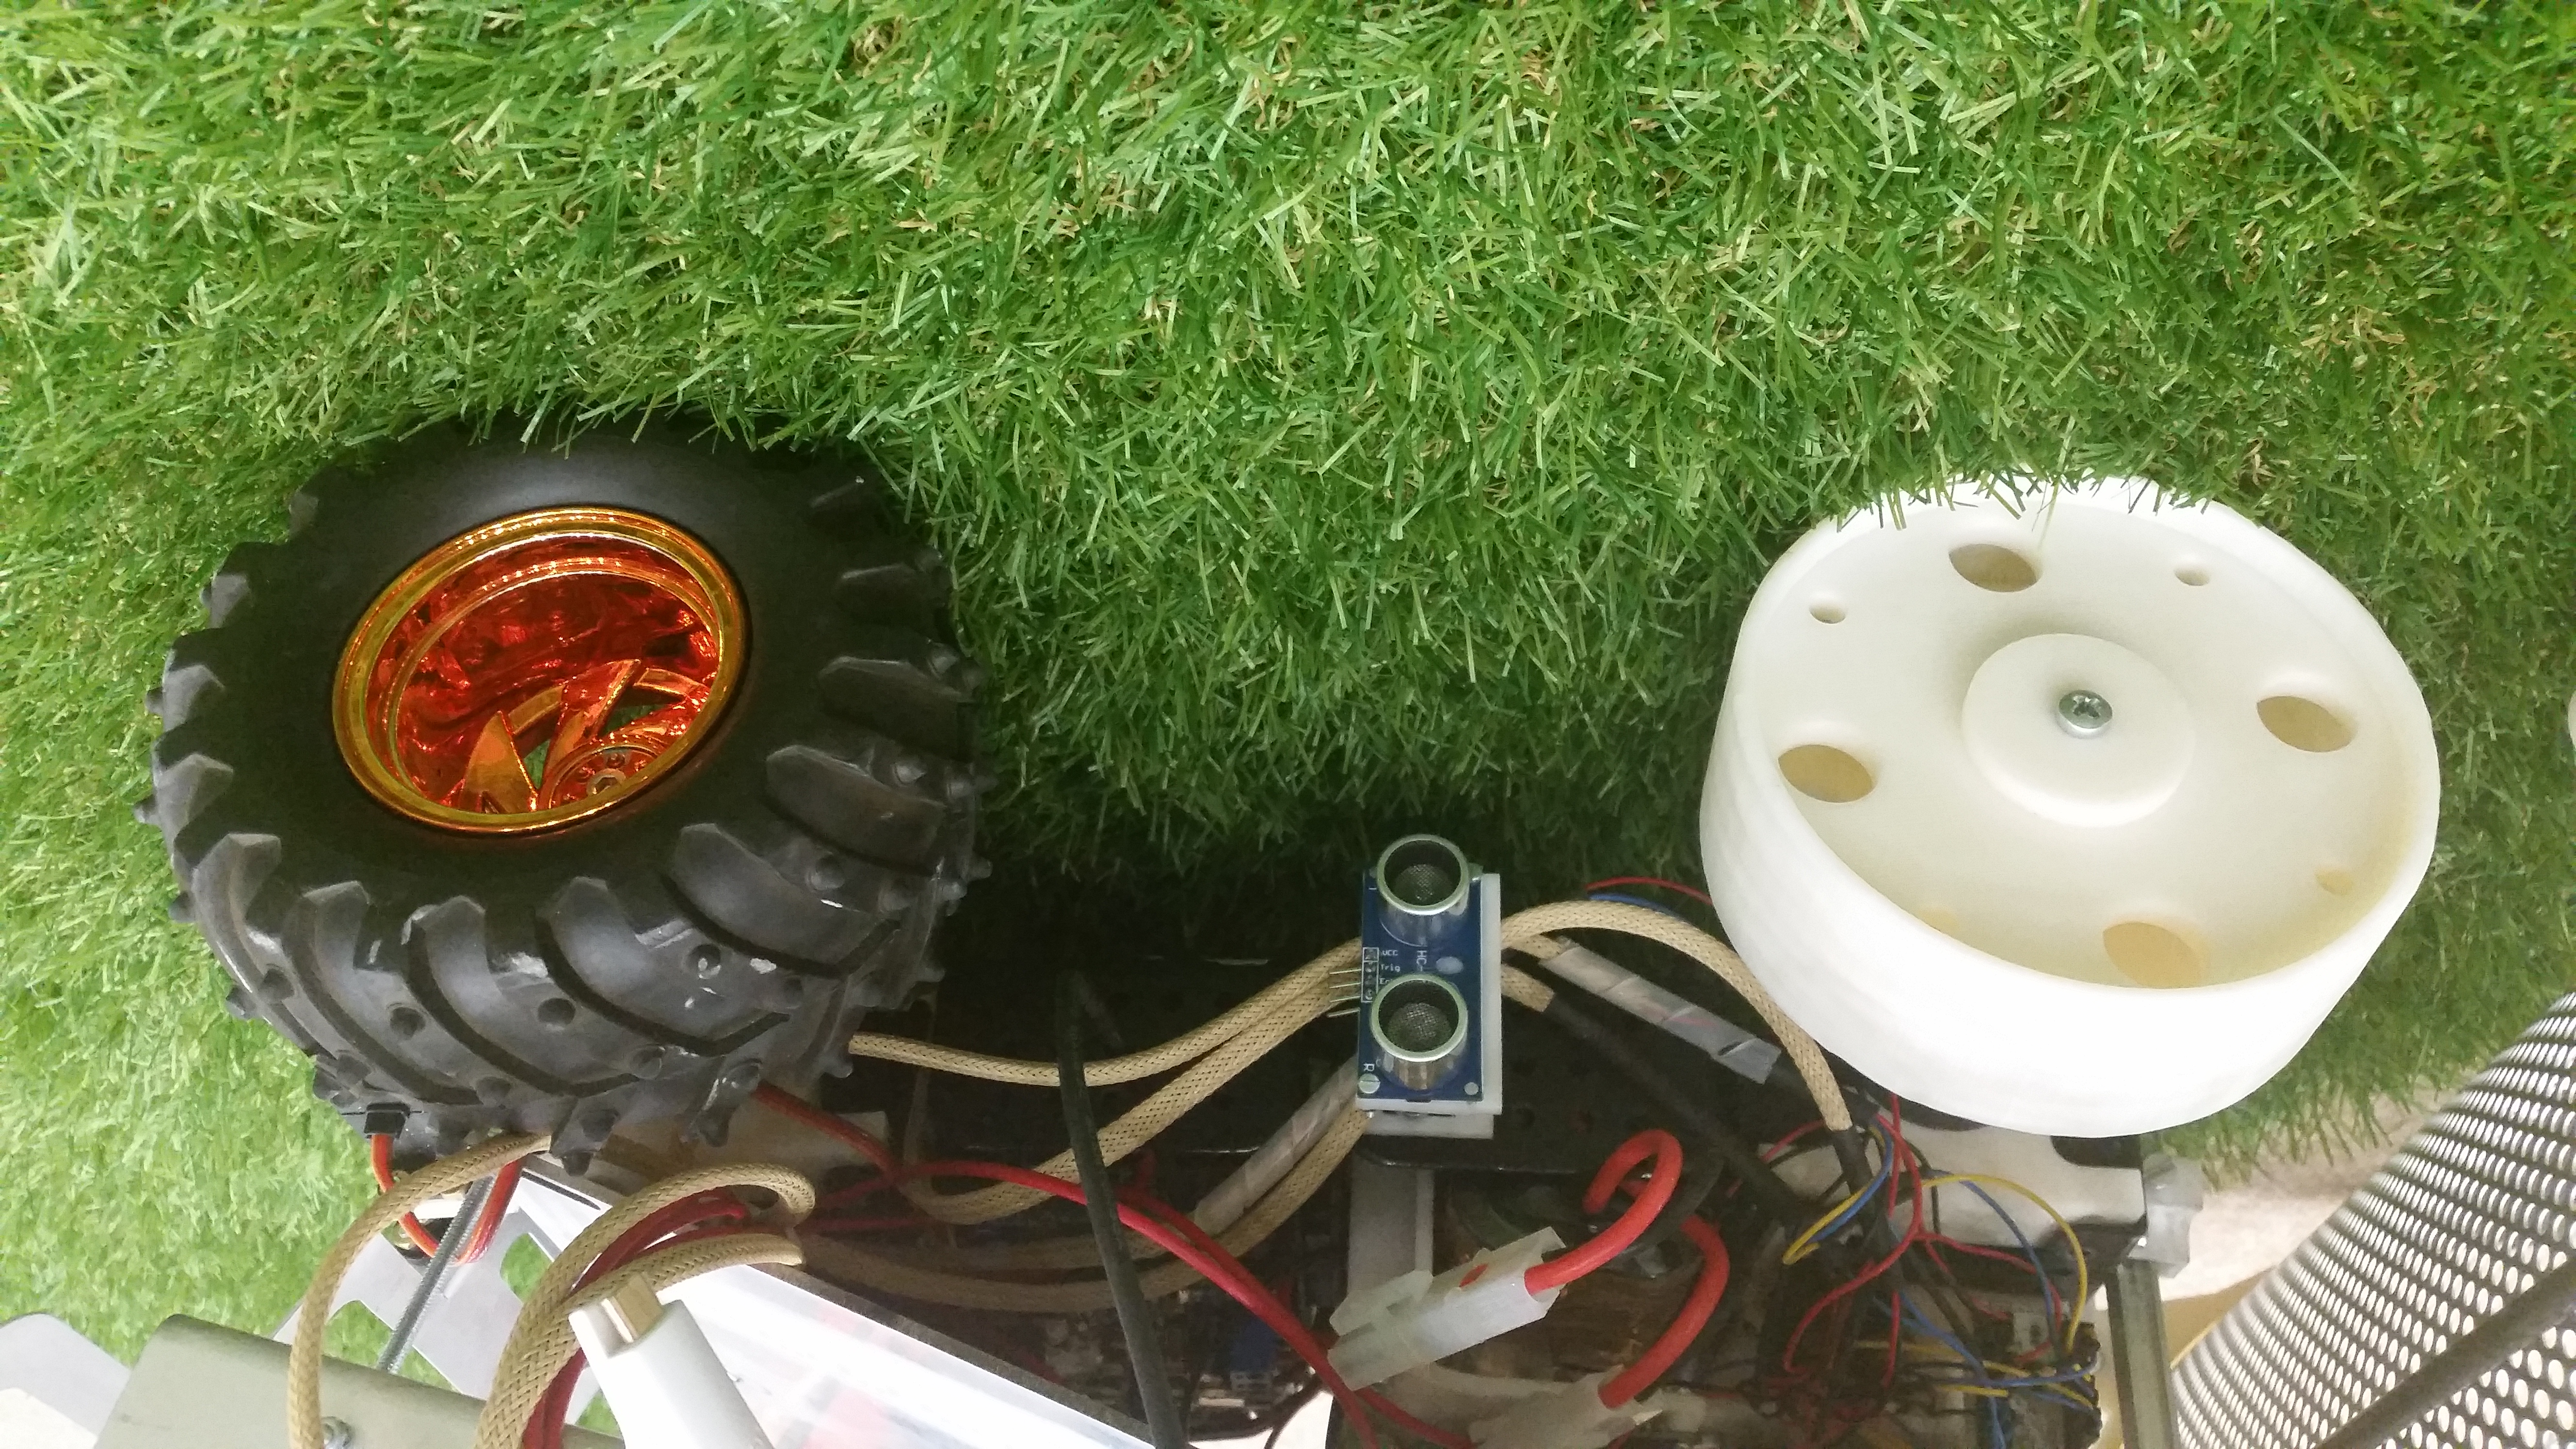
\includegraphics[width=0.3\textwidth]{wheel.jpg}
  \caption{The 3D printed wheel, in comparison with a Wild thumper default wheel.}
\label{fig:wheel}
\end{figure}

%\textbf{And Lastly, a non-holonomic algorithm for the trajectory planning of the robot was implemented, so %that the robot would be able to move and rotate at the same time, reducing the stress on the wheelss.}

\section{Feedback speed Control}
A driver for the wild thumper was written, with the ability to count the pulses received from the encoders. However, as a replacement solution was found, the encoders were not used for the robot navigation.

\section{Tailgate}

To control the tailgate of the robot, in order to unload the bottles, a servo coupled to an aluminum plate was installed. 
As a Dynamixel AX-12A Smart servo was too powerful, we prefered to use a standart servo for this task.

\begin{figure}[H]
  \centering
  \includegraphics[width=0.3\textwidth]{servo.jpg}
  \caption{The 3001HB Servomotor.}
\label{fig:servo}
\end{figure}

With a torque of $4.4kg \cdot cm$, the 3001HB was the perfect servo for this task. As the torque needed was used only for the unloading of bottles, and the only stress on this motor was the gravity force of the bottles. 

The 3001HB serves perfectly it's purpose and has just the right amount of torque needed.

\section{Tests}

The testings were done in the beginning with the remote control, and later on with the wireless laptop control implemented on the Odroid. With the first tests a conclusion was made that the 75:1 gear motors were not powerful enough. Later with the higher gear ratio, the robot was slower but could move in an easier manner. On the grass, where the maximum friction, the robot was struggling to rotate, because of the position of the wheels, and the affected friction. After changing the front wheels with plastic cylinders, the robot could turn with ease, and no negative impact was found. 